\documentclass[letterpaper,journal]{IEEEtran}
\usepackage{amsmath,amsfonts}
\usepackage{algorithmic}
\usepackage{algorithm}
\usepackage{array}
\usepackage[caption=false,font=normalsize,labelfont=sf,textfont=sf]{subfig}
\usepackage{textcomp}
\usepackage{stfloats}
\usepackage{url}
\usepackage{graphicx}
\usepackage{cite}
\usepackage{booktabs}
\usepackage{multirow}
\usepackage{xcolor}
\usepackage{amssymb}
\usepackage{pifont}
\usepackage{microtype}
\Urlmuskip=0mu plus 6mu\relax
\hyphenation{op-tical net-works semi-conduc-tor IEEE-Xplore}

\begin{document}

\title{GeoViewMiner-SAM2: Geometry-Guided Satellite--UAV Fusion with Explicit Prompt Mining for Building Instance Segmentation}

\author{Anonymous~Author,~\IEEEmembership{Member,~IEEE}
\thanks{Manuscript submitted to IEEE JSTAR, July 2026.}}

\markboth{IEEE Journal of Selected Topics in Applied Earth Observations and Remote Sensing}%
{Author \MakeLowercase{\textit{et al.}}: GeoViewMiner-SAM2: Geometry-Guided Satellite--UAV Fusion}

\maketitle

\begin{abstract}
Remote sensing object instance segmentation is a core task in earth observation, yet the vast majority of existing methods operate exclusively on a single nadir-view satellite perspective. This single-stream paradigm suffers from inherent limitations: building boundaries are blurred by uniform roof materials, adjacent instances adhere at ground level, vertical facade structures remain invisible from overhead, and small or densely packed targets are frequently missed. Although cross-view learning between satellite and aerial imagery has attracted growing attention, existing cross-view efforts concentrate predominantly on visual geo-localization and image retrieval rather than instance-level segmentation, leaving the potential of multi-view fusion for dense per-instance mask prediction largely unexplored. In this work, we address these challenges through three main contributions. First, we propose \emph{PromptMiner-SAM2}, an automatic SAM2 Base+-based single-stream building instance segmenter that combines a PAFPN two-stage detector with explicit prompt construction. For each candidate instance, a supervised coarse mask is locally calibrated by a constrained residual predicted from high-resolution P2 features. The refined mask supplies adaptive foreground--background point prompts and a dense mask prompt, while the proposal box supplies the native SAM2 box prompt. The three prompt modalities are encoded by the frozen SAM2 PromptEncoder and guide the SAM2 MaskDecoder to produce the final instance mask. This satellite-side architecture is evaluated on WHU and forms the reference path of our dual-stream framework. Second, we construct \emph{SynSU-Build} (Synthetic Satellite--UAV Building Instance Segmentation Benchmark) from the Unreal Engine~5 (UE5) City Sample. It provides paired nadir satellite and multi-view oblique UAV RGB imagery, exact camera intrinsics and extrinsics, shared scene geometry, and pixel-accurate building instance annotations only for the satellite target view. Third, we propose \emph{GeoViewMiner-SAM2}, a ground-referenced multi-height cross-view ROI fusion model that lifts calibrated UAV features onto discrete world-height hypotheses, retrieves target-level information around satellite-derived ground anchors, and injects it into both box and mask ROI branches without requiring satellite camera parameters, depth, or building-height supervision. Extensive experiments on the WHU benchmark and SynSU-Build validate the effectiveness of each component and demonstrate the benefit of cross-view fusion for satellite-view building instance segmentation.
\end{abstract}

\begingroup
\hbadness=10000
\begin{IEEEkeywords}
Building instance segmentation, SAM2, PromptMiner-SAM2, GeoViewMiner-SAM2, satellite--UAV fusion, cross-view learning.
\end{IEEEkeywords}
\endgroup


%==============================================================================
\section{Introduction}
%==============================================================================
\IEEEPARstart{R}{emote} sensing object instance segmentation---the task of detecting and delineating each individual object instance in overhead imagery---is fundamental to a wide range of earth observation applications, including urban planning, disaster response, and map updating. Accurate building instance segmentation, in particular, underpins cadastral mapping, population estimation, and infrastructure monitoring. Despite significant progress, the field faces two persistent challenges: the limitations of the single-view paradigm, and the scarcity of geometrically reliable multi-view paired benchmarks designed for instance-level segmentation.

\subsection{Single-View Limitations and the Single-Stream Baseline}

Most remote sensing instance segmentation methods operate on a single nadir image. Region-based architectures such as Mask R-CNN and Cascade R-CNN~\cite{ref_maskrcnn,ref_cascade}, high-resolution variants such as HQ-ISNet~\cite{ref_hqisnet}, and query-based methods such as Mask2Former~\cite{ref_mask2former} have achieved strong results, but repeated downsampling and coarse mask prediction remain unfavorable for small buildings, weak boundaries, and touching instances. Promptable foundation models offer a powerful alternative segmentation prior: SAM~\cite{ref_sam} and SAM2~\cite{ref_sam2} can delineate objects from points, boxes, or masks. Their category-agnostic, interactive workflow, however, does not directly support automatic instance segmentation in dense overhead scenes. We adopt SAM2 because its hierarchical image encoder exposes multi-scale features that naturally support two-stage instance discovery while retaining the native prompt-conditioned mask decoder.

Automatic prompting methods such as RSPrompter~\cite{ref_rsprompter} remove manual interaction by generating learned prompt embeddings from region features. These embeddings connect instance detection to foundation-model decoding, but they do not explicitly supervise an intermediate instance shape or expose its geometry through native point and mask inputs. Our single-stream model instead predicts a supervised coarse mask for each candidate instance. The coarse prediction yields adaptive foreground--background points and a dense mask prompt, while the associated proposal supplies the box prompt. The resulting point, box, and mask inputs retain explicit meanings---interior and exclusion evidence, instance extent, and spatial support---and are encoded together by the frozen SAM2 PromptEncoder.

The coarse decoder establishes the overall instance shape from a fixed-resolution RoI feature, but its upsampled grid can smooth roof corners and narrow gaps. We therefore calibrate the coarse prediction before prompt construction with a P2BoundaryRefiner. For the same candidate box, the refiner extracts a higher-resolution P2 feature crop and predicts a bounded logit residual only inside a search band derived from the coarse boundary. It cannot rewrite confident interiors or recover regions outside this local support. The corrected geometry is then shared by point mining and dense-mask prompting, so high-resolution boundary evidence reaches the SAM2 decoder through both coarse-derived prompt routes. This design follows the broader principle that an initial mask contains useful structure for subsequent refinement~\cite{ref_pointrend,ref_cascadepsp,ref_segrefiner,ref_samrefiner}, while moving the correction before prompt encoding rather than applying it only to the final mask.

\subsection{Cross-View Pairing: The Data Gap}

Existing satellite--UAV datasets primarily support geo-localization and retrieval~\cite{ref_unigeo,ref_university}. They generally do not combine pixel-level building instances, exact cross-view correspondence, and camera parameters required for geometry-aware fusion. Collecting these elements in the real world is difficult: acquisition conditions differ substantially across platforms, metadata may be incomplete, and camera recovery can introduce scale, alignment, and reconstruction errors. Such uncertainty confounds geometric error with the model's actual use of UAV information.

Synthetic rendering provides controllable geometry and automatic annotation, as demonstrated by UrbanScene3D, UEMM-Air, and SynRS3D~\cite{ref_urbanscene3d,ref_uemmair,ref_synrs3d}. We therefore construct SynSU-Build from the UE5 City Sample, whose high-fidelity procedural city and World Partition system support large-scale, geometrically consistent urban rendering. We sample 4,000 valid urban centers in a shared metric world frame. At each center, one nadir satellite image is paired with five oblique UAV images distributed around the same ground target, so each sample provides complementary roof and facade observations rather than loosely matched geographic imagery.

The rendering pipeline records the complete intrinsic and extrinsic parameters of all five UAV cameras. Building meshes associated with the same City Sample anchor are consolidated into one satellite-view instance. Satellite RGB imagery and its instance-ID layer are rendered from the same camera frame, eliminating temporal and pose inconsistencies between images and labels. The five UAV views contain RGB imagery and camera parameters but no instance annotations. Consequently, SynSU-Build provides calibrated satellite--UAV observations together with pixel-accurate supervision only for the satellite target view. This controlled construction removes uncertain post-hoc camera recovery and manual cross-view alignment, allowing experiments to distinguish geometric failure from a model's inability to use UAV information.

\subsection{Cross-View Fusion: Toward Multi-View Instance Segmentation}
Simply concatenating satellite and UAV features does not ensure that the model uses geometrically relevant UAV information. The two platforms observe buildings under different scales and viewpoints, and the apparent satellite roof location may be displaced from a ground-plane correspondence by building height. A useful fusion mechanism must therefore tolerate uncertain height and local position while preserving the strong satellite-only prediction path.

We propose \emph{GeoViewMiner-SAM2}, the cross-view extension of PromptMiner-SAM2. Calibrated UAV features are projected onto a set of discrete world-height planes, producing a differentiable plane-sweep feature volume. A verified satellite pixel-to-ground affine supplies each satellite ROI with a coarse world-space anchor; the satellite ROI feature then retrieves UAV information over a restricted set of height and local horizontal-offset hypotheses. The retrieved spatial feature is injected through independently gated residuals into the bbox and mask ROI branches. The mask branch retains the complete PromptMiner-SAM2 prompt excavation and decoding chain, so UAV observations can influence the coarse shape, sparse and dense prompts, and final instance mask. The formulation requires UAV camera geometry and a coarse satellite ground mapping, but not satellite intrinsics/extrinsics, explicit depth, or building-height labels.

\subsection{Contributions}

The main contributions of this work are summarized as follows:
\begin{enumerate}
\item \textbf{PromptMiner-SAM2, a boundary-aware explicit-prompt architecture for remote sensing instance segmentation,} which learns a supervised coarse instance mask and converts it into adaptive foreground--background points and a dense mask prompt, complemented by a proposal-derived box prompt for the native frozen SAM2 PromptEncoder. Before prompt construction, a constrained P2 residual locally calibrates the coarse boundary and propagates the corrected geometry through both coarse-derived prompt routes. The architecture provides a controlled satellite-side reference path and supports separate evaluation of point, box, dense-mask, and boundary-refinement components.

\item \textbf{SynSU-Build, a fully synthetic satellite--UAV building instance segmentation benchmark,} constructed from the UE5 City Sample. SynSU-Build provides paired nadir satellite and five-view oblique UAV RGB imagery, exact camera intrinsics and extrinsics, a shared metric world frame, and pixel-level building masks only for the satellite target view, enabling controlled training and causal evaluation without uncertain post-hoc camera reconstruction.

\item \textbf{GeoViewMiner-SAM2, a geometry-guided satellite--UAV dual-stream model,} which lifts calibrated UAV features to discrete world-height hypotheses, performs ground-anchored local height--position retrieval for each satellite ROI, and independently enhances bbox and mask features through conservative gated residuals. The method requires neither satellite camera parameters nor explicit depth or building-height supervision.
\end{enumerate}

The remainder of this paper is organized as follows. Section~\ref{sec:related} reviews related work. Section~\ref{sec:method} presents the single-stream model, SynSU-Build construction, and dual-stream fusion framework in sequence. Section~\ref{sec:experiments} presents the experimental setup and results, Section~\ref{sec:discussion} discusses the main findings, and Section~\ref{sec:conclusion} concludes the paper.

% Reserve the remainder of page 2 for the forthcoming Section I-C text.
\clearpage

%==============================================================================
\section{Related Work}
\label{sec:related}
%==============================================================================

\subsection{Remote Sensing Instance Segmentation}
Remote sensing instance segmentation initially followed general-purpose two-stage detectors. Mask R-CNN~\cite{ref_maskrcnn} adds an ROI mask head to object detection, while Cascade R-CNN and HTC~\cite{ref_cascade,ref_htc} progressively improve localization through cascaded stages. Remote-sensing-specific designs such as HQ-ISNet~\cite{ref_hqisnet} strengthen high-resolution and multi-scale feature propagation for small, densely distributed targets. Boundary-oriented methods take a complementary direction: PointRend~\cite{ref_pointrend} adaptively updates uncertain pixels, whereas polygon-based P2PFormer~\cite{ref_p2pformer} directly predicts ordered building contours. Query-based architectures such as Mask2Former~\cite{ref_mask2former} further replace proposal-wise classification with global mask queries and masked attention.

Despite this progress, each formulation retains limitations in overhead building scenes. RoI mask heads predict on fixed-resolution grids and can smooth corners or merge touching roofs; cascaded detection improves boxes without necessarily recovering mask detail; query-based models require substantial task-specific supervision; and polygon methods depend on reliable corner ordering and topology. These weaknesses become pronounced under large scale variation, weak roof contrast, narrow gaps, and dense settlements. Promptable foundation models offer a complementary mask prior, but their interactive, category-agnostic interfaces do not by themselves discover and classify all instances in an image. Automatic instance segmentation therefore requires a detection mechanism together with a proposal-conditioned interface to the foundation-model decoder.

\subsection{Foundation Models for Remote Sensing}
Early studies investigated whether SAM could transfer directly to aerial and satellite imagery through zero-shot or lightly adapted prompting. Osco \textit{et al.}~\cite{ref_samrsapp} evaluated point-, box-, and text-guided SAM across remote sensing scales, demonstrating its potential but also its sensitivity to spatial resolution and prompt design. Data-centric work followed: SAMRS~\cite{ref_samrs} combines existing detection annotations with SAM to generate more than one million remote sensing masks for segmentation pre-training. Other methods use SAM outputs as auxiliary priors rather than as the final instance predictor. For example, SAM-assisted semantic segmentation~\cite{ref_samassist} extracts SAM-generated objects and boundaries to impose region-consistency and boundary constraints on a conventional semantic segmentation network. These approaches improve annotation scalability or semantic segmentation, but they do not directly resolve automatic category-aware instance localization and per-instance prompting.

For remote sensing instance segmentation, learned-prompt approaches map proposal features to prompt embeddings and thereby remove manual interaction~\cite{ref_rsprompter}. Other methods adapt the foundation model itself: MC-SAM SEG~\cite{ref_mcsamseg} inserts multi-cognitive visual adapters into the SAM encoder and uses pixel and transformer decoders for prompt-free mask classification, while RS4D~\cite{ref_rs4d} distills foundation-model knowledge into a state-space backbone to reduce the cost of dense instance prediction. These directions respectively emphasize automatic interaction, domain adaptation, and efficient knowledge transfer. Our focus is different: we preserve the native geometric prompt interface and construct its point, box, and mask inputs explicitly for each detected instance.

A closely related line of research treats an initial coarse mask as structured input for a subsequent refinement stage. CascadePSP~\cite{ref_cascadepsp} combines global and local image evidence to refine low-resolution masks at high resolution, while SegRefiner~\cite{ref_segrefiner} formulates model-agnostic mask refinement as progressive denoising with a discrete diffusion process. More directly related to promptable foundation models, SAMRefiner~\cite{ref_samrefiner} excavates distance-guided points, context-aware elastic boxes, and Gaussian-style masks from a pre-existing coarse mask before invoking SAM. In these formulations, the initial mask is supplied by an upstream predictor and refinement is applicable independently of that predictor. In our model, by contrast, the coarse mask is learned internally from proposal-aligned detection features and supervised jointly with the instance segmentation task. It serves as the shared source for adaptive foreground--background points and a dense mask prompt. P2BoundaryRefiner further modifies this source only within a prediction-derived boundary neighborhood, placing local correction before prompt encoding instead of refining only the final output.

PromptMiner-SAM2 therefore uses SAM2 Base+ for both hierarchical detection features and the image representation consumed by its mask decoder. PAFPN organizes the hierarchical features for RPN proposal generation, box recognition, and proposal-wise mask feature extraction. Each mask feature predicts a supervised coarse instance mask; its P2-calibrated geometry yields adaptive foreground--background points and a dense mask input, while the proposal supplies the box input. The frozen native PromptEncoder encodes these explicit modalities, and the SAM2 MaskDecoder produces the final instance mask from the resulting prompts and shared image features.

\subsection{Synthetic Data for Remote Sensing}
Synthetic rendering has become an important alternative when aerial acquisition, camera calibration, or dense annotation is expensive. Synthinel-1~\cite{ref_synthinel} generates overhead urban imagery and building labels for studying synthetic-to-real transfer. UrbanScene3D~\cite{ref_urbanscene3d} combines real reconstructed regions with Unreal Engine and AirSim environments, providing controllable flight patterns, depth, LiDAR, bounding boxes, and building identities for aerial perception and reconstruction. SkyScenes~\cite{ref_skyscenes} expands viewpoint and environmental diversity with densely labeled UAV scenes, while UEMM-Air~\cite{ref_uemmair} produces aligned multimodal UAV observations for multiple perception tasks. At the satellite scale, SynRS3D~\cite{ref_synrs3d} supports land-cover mapping, height estimation, and building change analysis through globally diverse synthetic scenes. GTA-UAV~\cite{ref_gtauav} further demonstrates that game environments can generate large contiguous UAV--satellite regions for cross-view localization.

These datasets establish the value of exact rendering geometry and automatic labels, but they are typically organized around a single viewpoint, semantic categories, 3D reconstruction, or image-level geo-localization. They do not simultaneously provide calibrated paired satellite--UAV imagery and instance supervision for the satellite target view. SynSU-Build addresses this combination using controlled rendering in the UE5 City Sample: its UAV component contains only RGB images and camera parameters, while detection and mask annotations are provided exclusively for the paired satellite image. Rather than using synthetic images only as additional training samples, the benchmark isolates geometric alignment, appearance variation, and UAV information utilization in satellite-view instance segmentation. Its controllability also enables counterfactual tests with correct, shifted, or bypassed UAV inputs, which are difficult to construct reliably from real acquisitions.

\subsection{Cross-View Learning}
Cross-view learning first developed around image retrieval and geo-localization. University-1652~\cite{ref_university} introduced matched satellite, synthetic UAV, and ground observations for drone-view target localization and navigation. TransGeo~\cite{ref_transgeo} replaced hand-crafted polar alignment with a transformer that models global cross-view correlations, while DenseUAV~\cite{ref_denseuav} moved toward real low-altitude urban imagery, dense spatial sampling, and joint retrieval/localization evaluation. Subsequent UAV--satellite methods continue to improve viewpoint-invariant representations, scale handling, and pose estimation. Nevertheless, their supervision is dominated by image-level identity, retrieval ranking, or geographic position. Such objectives can identify \emph{where} a UAV image was captured without learning pixel-accurate correspondence between UAV observations and individual satellite-view buildings.

A second line of work transforms perspective observations into a canonical top-down representation. Cross-View Transformers~\cite{ref_cvt} use camera-aware attention to infer map-view semantic segmentation from calibrated multi-camera images. In a remote sensing context, SG-BEV~\cite{ref_sgbeyv} projects street-view features into BEV space and fuses them with satellite features for fine-grained building-attribute semantic segmentation. These methods demonstrate the value of geometric intermediates and dense cross-view fusion, but their outputs are semantic maps. They also rely on datasets designed for retrieval or semantic labeling rather than paired satellite--UAV observations with camera geometry and satellite-view instance masks.

Our setting differs in both output and evaluation. UAV views are auxiliary observations, whereas the required output is a set of detection boxes and per-building masks in the satellite view. Cross-view features must therefore preserve local geometry, associate with individual satellite proposals, and improve prediction only when the paired UAV information is relevant. This motivates not only geometry-aware feature projection but also counterfactual diagnostics that distinguish genuine cross-view information use from improvements caused by additional parameters or confidence bias.

\section{Method}
\label{sec:method}
%==============================================================================

\subsection{PromptMiner-SAM2: Explicit Prompt Mining from Coarse Shapes}
\label{sec:single_method}

PromptMiner-SAM2 turns the interactive SAM2 image-segmentation pipeline into an automatic building instance segmenter. Its standard detection path discovers candidate instances, while two proposed modules construct explicit prompts: an \emph{Explicit Coarse-Prompt Miner} learns proposal-conditioned instance geometry and converts it into native SAM2 prompts, and \emph{P2BoundaryRefiner} locally calibrates that geometry before prompt construction. The resulting prompts are processed by the pretrained PromptEncoder and the SAM2 MaskDecoder.

\subsubsection{Overall Architecture}
For a $1024\times1024$ image, the SAM2 Hiera-Base+ image encoder produces four 256-channel hierarchical maps at strides $\{4,8,16,32\}$. This representation is a principal reason for adopting SAM2: unlike a single terminal feature map, the hierarchy naturally supplies the spatial scales required by a two-stage detector. A detection-oriented PAFPN applies top-down and bottom-up fusion and outputs five 512-channel levels $\{P_2,\ldots,P_6\}$ at strides $\{4,8,16,32,64\}$. An RPN generates proposals, and a Shared2FC bounding-box head performs building classification and box regression. In parallel, we retain the stride-16 $64\times64$ SAM2 image embedding and the two higher-resolution encoder features used by the native MaskDecoder. A single pretrained image encoder therefore supports both automatic instance discovery and prompt-conditioned segmentation.

Let $b_r$ denote the candidate box used by the mask branch: a sampled positive proposal during training and a final detected box during inference. Multi-level RoIAlign extracts a $14\times14$ mask feature $X_r\in\mathbb{R}^{512\times14\times14}$ from $P_2$--$P_5$. The same $b_r$ defines the coordinate frame for mask feature extraction, coarse-mask supervision, point-coordinate conversion, dense-mask placement, and the SAM2 box prompt. This shared geometry keeps all prompt modalities aligned with the instance being decoded.

\subsubsection{Module I: Explicit Coarse-Prompt Miner}
The first proposed module represents each candidate instance with an explicitly supervised intermediate mask rather than mapping $X_r$ directly to unconstrained prompt embeddings. A lightweight convolutional decoder with two upsampling stages predicts
\begin{equation}
C_r=f_{\mathrm{coarse}}(X_r), \qquad
C_r\in\mathbb{R}^{1\times64\times64}.
\label{eq:coarse_logits}
\end{equation}
The corresponding ground-truth instance is cropped by $b_r$ and resized to the same grid. Binary cross-entropy and Dice losses supervise $C_r$, making the intermediate geometry inspectable and independent of the final decoder output.

The module converts the boundary-calibrated logits $\widehat C_r$ defined below into complementary sparse and dense prompts. For sparse prompting, an adaptive 2P2N miner selects at most two foreground and two background points. The first positive favors a confident location with large interior distance, and the second is required to be spatially separated. Background points are sought first near the predicted outer boundary and then in a separated, low-confidence background region. Confidence, topology, and distance tests determine the validity of each point; invalid entries are neutralized, and an instance with no reliable point falls back to its remaining prompt modalities. Valid local coordinates are mapped to image coordinates through $b_r$. The same box supplies SAM2's native two-corner box prompt.

For dense prompting, the coarse logits are resized and placed inside $b_r$ on the native mask-input canvas of the PromptEncoder,
\begin{equation}
Q_r=\operatorname{Place}(\widehat C_r,b_r).
\label{eq:dense_canvas}
\end{equation}
Let $E_r^{\mathrm{mask}}$ be the mask embedding produced by the frozen PromptEncoder, $E^0$ its pretrained no-mask embedding, and $M_r$ the box support at the dense-embedding resolution. The dense embedding supplied to the MaskDecoder is
\begin{equation}
D_r=E^0+\alpha M_r\odot
\left(E_r^{\mathrm{mask}}-E^0\right),
\qquad \alpha=\sigma(a),
\label{eq:dense_prompt_gate}
\end{equation}
where the learnable global gate is initialized with $\alpha=0.25$. The support mask confines the learned dense correction to the candidate box. Points, the box, and $Q_r$ are passed together through a single frozen PromptEncoder call, preserving their native SAM2 semantics while providing interior, exclusion, extent, and shape evidence.

\subsubsection{Module II: P2BoundaryRefiner}
The coarse decoder must infer the complete instance shape from a fixed $14\times14$ RoI feature. P2BoundaryRefiner therefore introduces higher-resolution evidence without allowing an unconstrained second mask predictor. Let $F_2=P_2$ and $\operatorname{sg}(\cdot)$ denote stop-gradient. From the raw coarse prediction it computes
\begin{equation}
p_r=\sigma(\operatorname{sg}(C_r)), \qquad
u_r=4p_r(1-p_r), \qquad
S_r=\mathcal{B}(p_r),
\label{eq:p2_support}
\end{equation}
where $\mathcal{B}$ applies $3\times3$ smoothing, thresholds the result at 0.5, extracts its morphological boundary, and dilates that boundary by four coarse-grid pixels. The support is generated from the prediction alone. It is disabled when empty or when it covers more than half of the coarse canvas, preventing local calibration from becoming a global rewrite.

A learned $1\times1$ projection reduces $F_2$ from 512 to 64 channels before a $32\times32$ RoIAlign crop is extracted at $b_r$. With
\begin{equation}
Z_r=\operatorname{RoIAlign}(\Pi_2(\operatorname{sg}(F_2)),b_r),
\qquad
H_r=Z_r-\operatorname{AvgPool}_{3\times3}(Z_r),
\end{equation}
the refiner fuses $Z_r$, its high-frequency component $H_r$, resized $p_r$ and $u_r$, and the search support. Two convolutional blocks followed by a residual head predict
\begin{equation}
\begin{aligned}
\Delta_r&=0.20\,[2\tanh(h_{\mathrm{P2}}(
Z_r,H_r,p_r,u_r,S_r))]\odot S_r,\\
\widehat C_r&=C_r+\Delta_r.
\end{aligned}
\label{eq:p2_refinement}
\end{equation}
Thus $\Delta_r\in[-0.4,0.4]$ and is zero outside $S_r$. The residual head is zero initialized, so enabling the module initially leaves the coarse prediction unchanged. The raw coarse mask remains responsible for topology and overall extent; P2BoundaryRefiner can only calibrate a neighborhood supported by its predicted boundary. During training, a local boundary BCE supervises $\operatorname{sg}(C_r)+\Delta_r$ inside valid search regions and is normalized over valid instances.

\subsubsection{Prompt-Conditioned Decoding and Objective}
For every candidate instance, the frozen PromptEncoder returns sparse embeddings for the valid points and box corners and a mask embedding for $Q_r$; Eq.~\eqref{eq:dense_prompt_gate} then forms the gated dense embedding $D_r$. The corresponding stride-16 image embedding is reused across all instances in the image, while the two higher-resolution SAM2 features are repeated in the same instance order. The trainable SAM2 MaskDecoder consumes these image features, positional encoding, and prompt embeddings to predict one mask per candidate. During inference, the predicted mask is mapped through its detected box to the image canvas and thresholded using the common evaluation configuration.

The complete single-stream objective is
\begin{equation}
\mathcal{L}=\mathcal{L}_{\mathrm{det}}
+\mathcal{L}_{\mathrm{mask}}
+0.10\mathcal{L}_{\mathrm{coarse}}
+0.05\mathcal{L}_{\mathrm{p2}}.
\label{eq:single_loss}
\end{equation}
Here $\mathcal{L}_{\mathrm{det}}$ contains the RPN classification and regression losses and the RoI classification and box-regression losses. $\mathcal{L}_{\mathrm{mask}}$ is the standard per-pixel binary mask loss for the assigned instance, $\mathcal{L}_{\mathrm{coarse}}$ combines binary cross-entropy and Dice losses on the raw coarse prediction, and $\mathcal{L}_{\mathrm{p2}}$ is the valid-instance-normalized local boundary BCE. The latter uses ground truth only in its training loss; the refinement support used in both training and inference is derived solely from the raw prediction.

%==============================================================================
\subsection{SynSU-Build Dataset Construction}
\label{sec:dataset}
%==============================================================================

Table~\ref{tab:dataset_comparison} compares SynSU-Build with representative cross-view and synthetic remote sensing datasets. Existing satellite--UAV datasets mainly support image retrieval or geo-localization, whereas synthetic aerial datasets provide controllable views or dense labels without paired satellite observations. SynSU-Build combines calibrated paired imagery and multiple UAV viewpoints with building instance masks for the satellite target view.

\begin{table*}[!t]
\caption{Comparison with Representative Cross-View and Synthetic Remote Sensing Datasets}
\label{tab:dataset_comparison}
\centering
\scriptsize
\setlength{\tabcolsep}{3.2pt}
\renewcommand{\arraystretch}{1.12}
\begin{tabular*}{\textwidth}{@{\extracolsep{\fill}}lccccccl@{}}
\toprule
Dataset & Source & Views & S--U Pair & Multi-UAV & Camera Geom. & Sat. Inst. Masks & Primary Task \\
\midrule
University-1652~\cite{ref_university} & Hybrid & S/U/G & \ding{51} & \ding{51} & \ding{55} & \ding{55} & Geo-localization \\
DenseUAV~\cite{ref_denseuav} & Real & S/U & \ding{51} & \ding{51} & $\triangle$ & \ding{55} & Geo-localization \\
GTA-UAV~\cite{ref_gtauav} & Synthetic & S/U & $\triangle$ & \ding{51} & $\triangle$ & \ding{55} & Geo-localization \\
UrbanScene3D~\cite{ref_urbanscene3d} & Hybrid & U/3D & \ding{55} & \ding{51} & \ding{51} & \ding{51} & Reconstruction/3D inst. \\
SkyScenes~\cite{ref_skyscenes} & Synthetic & U & \ding{55} & \ding{51} & $\triangle$ & \ding{51} & Scene understanding \\
UEMM-Air~\cite{ref_uemmair} & Synthetic & U/MM & \ding{55} & \ding{51} & $\triangle$ & \ding{55} & Object detection \\
SynRS3D~\cite{ref_synrs3d} & Synthetic & S & \ding{55} & \ding{55} & $\triangle$ & \ding{55} & Semantic/height \\
\midrule
\textbf{SynSU-Build} & Synthetic & S/U & \ding{51} & \ding{51} & \ding{51} & \ding{51} & Instance segmentation \\
\bottomrule
\multicolumn{8}{l}{\footnotesize S: satellite; U: UAV; G: ground; MM: multimodal.} \\
\multicolumn{8}{l}{\footnotesize \ding{51}: available; \ding{55}: unavailable; $\triangle$: partial correspondence or pose metadata only.}
\end{tabular*}
\end{table*}

\noindent\textit{Scene and spatial sampling.}
We build SynSU-Build on the UE5 City Sample, an official technical demonstration containing a large, detailed urban environment~\cite{ref_citysample}. UE5 World Partition divides this environment into streamable spatial cells while preserving a shared world coordinate system~\cite{ref_worldpartition}. The combination of contiguous city coverage, stable building actors, programmable cameras, and deterministic rendering enables paired satellite--UAV acquisition and direct generation of satellite-view instance labels.

Valid urban regions are traversed using a 200-m coarse grid, with up to 25 candidate ground locations placed inside each grid cell. Actor-based probes reject candidates with insufficient nearby urban content, yielding 4,000 sampling centers in a shared metric world coordinate system. This procedure provides broad spatial coverage while avoiding empty or weakly urbanized regions.

Figure~\ref{fig:sampling_pipeline} illustrates the spatial sampling strategy, the satellite--UAV camera arrangement, and the satellite-view instance annotations generated for each accepted center.

% Fig. 1 is reserved for the forthcoming single-stream architecture diagram.
\setcounter{figure}{1}
\begin{figure}[!t]
\centering
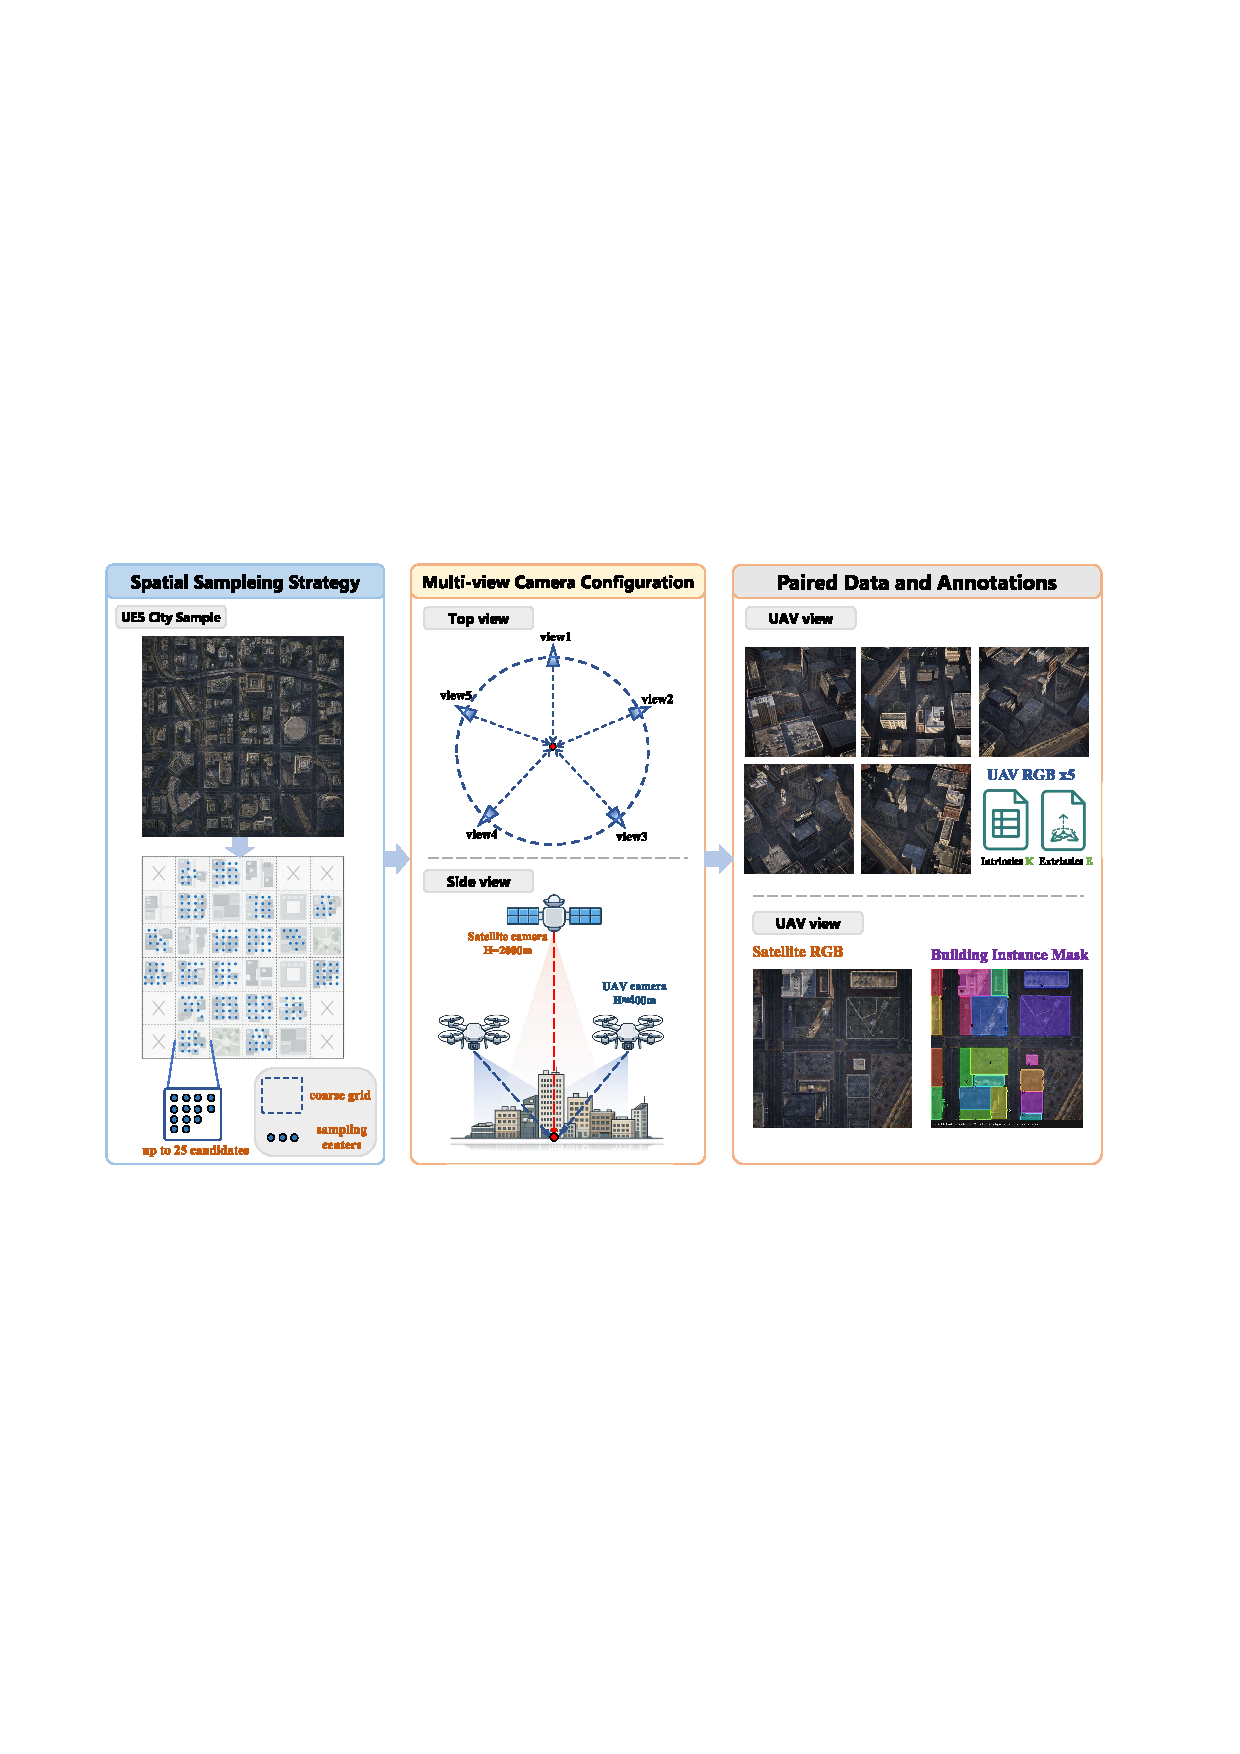
\includegraphics[width=\columnwidth]{采样示例图.pdf}
\caption{Overview of the SynSU-Build sampling and rendering pipeline. Left: urban sampling centers are selected using coarse spatial cells, multiple within-cell candidates, and actor-based content filtering. Middle: one nadir satellite camera and five oblique UAV cameras observe a common ground center. Right: each accepted sample contains five unannotated UAV RGB images with camera parameters and a paired satellite RGB image with its building instance mask.}
\label{fig:sampling_pipeline}
\end{figure}

\noindent\textit{Camera configuration.}
At each sampling center, we render five oblique UAV views at uniformly spaced azimuths of $0^{\circ}$, $72^{\circ}$, $144^{\circ}$, $216^{\circ}$, and $288^{\circ}$. The cameras lie on a 300-m horizontal orbit at a nominal altitude of 400~m and observe the same ground center, with a deterministic pitch perturbation within $\pm5^{\circ}$ to introduce controlled viewpoint variation. Each UAV camera uses a 55.4-mm focal length, a 36-mm square sensor, and a resolution of $512\times512$ pixels. A paired nadir satellite view is captured directly above the ground center from an altitude of 2,000~m using a 200-mm focal length. Intrinsic and extrinsic parameters are exported independently for all six views, providing exact cross-view geometry without post-hoc camera reconstruction.

\noindent\textit{Instance annotation.}
City Sample buildings can comprise multiple mesh actors. We group actors associated with the same building anchor into one satellite-view instance and assign a frame-local label for rendering. Satellite RGB and instance-ID layers are produced from the same Movie Render Queue camera frame, preventing pose or timing misalignment between imagery and labels. The integer-preserving ID layers are exported as linear OpenEXR files and subsequently converted into binary instance masks, bounding boxes, areas, and COCO-format annotations. No pixel-level instance-ID correspondence across satellite and UAV views is provided or used by the model.

\noindent\textit{Split and quality control.}
For scalable production, runtime Level Sequences and a PIE executor combine five consecutive sampling centers into each rendering job. Sample-level state tracking, camera-pose checks, image-statistics thresholds, and checkpoint-based recovery support automatic acceptance and interrupted-job resumption. SynSU-Build is divided using spatially disjoint urban blocks to prevent nearby or overlapping regions from appearing across training, validation, and test sets. Before release and final reporting, we audit complete six-view availability, camera matrices, RGB/EXR correspondence, valid projected coverage, non-empty satellite masks, and per-image instance statistics. Final accepted sample counts, split sizes, building totals, and rejection causes will be inserted after the full production audit.

%==============================================================================
\enlargethispage{\baselineskip}
\subsection{GeoViewMiner-SAM2}
\label{sec:dual_method}
%==============================================================================

GeoViewMiner-SAM2 retains the complete PromptMiner-SAM2 satellite network and introduces UAV information only after satellite ROI extraction. This design treats PromptMiner-SAM2 as a stable reference path: the satellite encoder, PAFPN, RPN, box head, coarse-prompt generator, P2BoundaryRefiner, PromptEncoder, and SAM2 MaskDecoder remain unchanged. The UAV branch supplies bounded residual features to the bbox and mask ROI streams, allowing cross-view information to improve both localization and delineation without replacing the satellite representation.

\subsubsection{Geometric Conditions and Multi-Height UAV Volume}
For each satellite image, the auxiliary input comprises $V$ calibrated UAV views $\{I_v,K_v,E_v\}_{v=1}^{V}$, where $K_v$ and $E_v$ denote the UAV intrinsic and world-to-camera extrinsic matrices. No satellite camera model is assumed. Instead, a verified affine transform maps original satellite pixels to ground-plane world coordinates. This mapping is deliberately interpreted as a coarse ground reference rather than an exact correspondence between elevated roof pixels and three-dimensional surfaces.

Because neither depth nor building height is available, we represent UAV information using a set of nonuniform height hypotheses $\mathcal{H}=\{z_k\}_{k=1}^{K}$. For every location $(X_i,Y_j)$ on a common world grid, the point $P_{ijk}=(X_i,Y_j,z_k,1)^{\top}$ is projected into UAV view $v$ as
\begin{equation}
p_{vijk}=\pi\!\left(K_vE_vP_{ijk}\right),
\end{equation}
where $\pi(\cdot)$ performs perspective division. Bilinear sampling obtains the corresponding feature from each UAV image, and valid observations are aggregated across views:
\begin{equation}
V_k(i,j)=
\frac{\sum_v a_{vijk}F_v(p_{vijk})}
{\sum_v a_{vijk}+\epsilon}.
\label{eq:height_volume}
\end{equation}
Here $a_{vijk}$ masks invalid projections and may incorporate view reliability. Alongside the feature volume, we retain coverage, valid-view count, and cross-view consistency statistics. The resulting representation is a differentiable plane-sweep height-hypothesis volume; it is neither a depth map nor a three-dimensional occupancy reconstruction. Its purpose is to expose alternative geometric explanations to the downstream task, which learns which heights are useful through detection and mask supervision.

\subsubsection{Ground-Referenced ROI Candidate Retrieval}
Each satellite ROI is mapped to the UAV world frame through the ground affine. When satellite images have been resized or augmented, the complete ROI sampling grid is first transformed back to original image coordinates, preserving its orientation and spatial layout. The affine then yields a coarse ground anchor for the ROI. Since elevated roofs need not align exactly with this anchor, we search a small neighborhood of horizontal offsets $\mathcal{D}=\{\Delta_m\}_{m=1}^{M}$ jointly with the height hypotheses.

A pooled satellite ROI feature forms the query $q_r$. For each pair $(z_k,\Delta_m)$, a low-cost token $t_{rkm}$ is sampled from the corresponding region of the UAV volume. Candidate relevance is computed as
\begin{equation}
s_{rkm}=
\frac{\phi_q(q_r)^{\top}\phi_k(t_{rkm})}{\sqrt{d}}
b^{h}_{k}+b^{c}_{rkm}+b^{a}_{rkm},
\label{eq:candidate_score}
\end{equation}
where $b^{h}_{k}$ is a learned height prior, while $b^{c}_{rkm}$ and $b^{a}_{rkm}$ encode projection coverage and cross-view agreement. Candidates without valid UAV coverage are masked before a joint softmax over height and position:
\begin{equation}
P_{rkm}=\operatorname{Softmax}_{k,m}(s_{rkm}).
\end{equation}
Coverage indicates only whether a hypothesis projects into valid UAV images; it is not interpreted as physical visibility or absence of occlusion.

Rather than selecting a hard top-$K$ candidate during training, we preserve gradient flow through a soft spatial retrieval. The marginal weight of height $k$ and its expected horizontal correction are
\begin{equation}
w_{rk}=\sum_mP_{rkm}, \qquad
\bar{\Delta}_{rk}=
\frac{\sum_mP_{rkm}\Delta_m}{w_{rk}+\epsilon}.
\end{equation}
One full spatial crop $C_{rk}$ is then sampled from each height plane at the corrected ROI location, and the target-level UAV feature is
\begin{equation}
U_r=\phi_v\!\left(\sum_k w_{rk}
\operatorname{GridSample}(V_k,B_r+\bar{\Delta}_{rk})\right).
\label{eq:uav_roi}
\end{equation}
This factorization evaluates all coarse height--position hypotheses using inexpensive tokens but extracts only one spatial crop per height. It therefore preserves the spatial structure needed by instance masks without expanding every candidate into a full ROI feature.

\subsubsection{BBox and Mask ROI Residual Fusion}
Bbox and mask branches use different ROI sets and spatial resolutions: the bbox head operates on sampled positive and negative proposals, whereas the mask branch processes positive refined boxes during training and final detections during inference. We consequently perform retrieval separately for the two branches. For branch $l\in\{b,m\}$, the fused feature is
\begin{equation}
F'_{r,l}=F_{r,l}+\alpha_lG_{r,l}\odot U_{r,l},
\label{eq:dual_residual}
\end{equation}
where $G_{r,l}$ is a branch-specific gate and $\alpha_l$ is a bounded learnable residual scale initialized near zero. If no height hypothesis has valid coverage, the residual is set exactly to zero, recovering the original satellite ROI feature.

The fused bbox feature is passed to the original classification and regression head, enabling UAV information to affect proposal scoring and box localization directly. The fused mask feature enters the unchanged explicit-prompt chain: coarse-mask prediction, P2 boundary residual refinement, adaptive foreground--background point mining, box and dense-mask prompt encoding, and final SAM2 mask decoding. UAV information can therefore influence the intermediate shape estimate and all derived prompts while retaining the same single-stream segmentation path. A strict bypass option disables both residual paths and provides an architecture-matched satellite-only control.

\subsubsection{Learning and Causal Diagnosis}
The cross-view modules are optimized jointly using the same detection, coarse-shape, and final-mask objectives defined for the single-stream model; no depth, height, occupancy, or explicit three-dimensional supervision is introduced. This makes task performance the only criterion for selecting useful height and offset hypotheses. To determine whether improvements genuinely depend on UAV information, evaluation holds the satellite image and ROI set fixed while replacing the auxiliary input with correctly paired, spatially shifted, far-scene, or bypassed UAV views. We report the candidate entropy, expected height and offset, valid-view coverage, branch gates, residual magnitude, and cross-view gradient norms together with the final AP metrics. Effective UAV utilization requires the correctly paired condition to outperform these counterfactual inputs and the architecture-matched satellite-only control.

\section{Experiments}
\label{sec:experiments}
%==============================================================================

\subsection{Datasets and Comparison Protocol}
\label{sec:experimental_datasets}

\noindent\textit{WHU Building Dataset.}
We use the original high-resolution version of the WHU building dataset~\cite{ref_whu} to evaluate PromptMiner-SAM2 on real aerial imagery. It contains 5,640 RGB images at $1024\times1024$ pixels, including 2,793 training images, 627 validation images, and 2,220 test images under the established instance-segmentation split~\cite{ref_p2pformer}. The dataset contains large variations in building scale, shape, density, roof appearance, and surrounding background. Because WHU does not provide paired UAV observations or camera geometry, it is used only for satellite-side instance segmentation and comparison with existing methods.

\noindent\textit{SynSU-Build.}
SynSU-Build is used to evaluate both satellite-only segmentation and satellite--UAV fusion. Each sample contains one $512\times512$ nadir satellite image, five calibrated $512\times512$ oblique UAV RGB images, and building instance annotations only for the satellite target view. The dataset is generated from 4,000 spatially sampled urban centers and is partitioned by disjoint spatial blocks; the final accepted train/validation/test counts will be reported after the production audit described in Section~\ref{sec:dataset}.

No previous method is designed for the same paired satellite--UAV instance-segmentation setting. We therefore retrain the comparison algorithms on the satellite RGB images and satellite-view masks only, so that all existing methods are evaluated as single-stream baselines under the same SynSU-Build split. PromptMiner-SAM2 uses the identical input protocol, whereas GeoViewMiner-SAM2 additionally receives the five UAV images and their camera parameters. This design separates gains from the satellite segmentation architecture from gains attributable to auxiliary UAV observations.

\noindent\textit{Counterfactual protocol.}
The counterfactual study will compare correctly paired, spatially shifted, far-scene, and strictly bypassed UAV inputs while holding the satellite image and evaluated ROI set fixed. Its quantitative results will be inserted after completion of the dual-stream experiments.

\subsection{Evaluation Metrics}
\label{sec:evaluation_metrics}
We use the standard COCO-style metrics for both bounding boxes and instance masks. For an intersection-over-union (IoU) threshold $t$, a prediction is counted as a true positive when it is matched to an unmatched ground-truth instance of the same category with
\begin{equation}
\operatorname{IoU}(P,G)=\frac{|P\cap G|}{|P\cup G|}\geq t,
\end{equation}
where $P$ and $G$ denote either two boxes or two binary masks. Predictions are sorted by confidence to obtain the precision--recall curve, and AP$_t$ is its interpolated area. We report AP$_{50}$ and AP$_{75}$ at IoU thresholds 0.50 and 0.75, respectively, together with the primary mean AP:
\begin{equation}
\operatorname{AP}=\frac{1}{10}\sum_{t\in\{0.50,0.55,\ldots,0.95\}}\operatorname{AP}_t.
\end{equation}
The prefixes \emph{bbox} and \emph{segm} distinguish box IoU from mask IoU. Single-stream checkpoints are selected by validation segm AP; bbox AP is tracked separately for localization analysis.

\subsection{Implementation Details and Main Results}
\label{sec:implementation_results}

\noindent\textit{Single-stream configuration.}
All images are resized to $1024\times1024$ pixels, with random horizontal flipping at probability 0.5 during training. PromptMiner-SAM2 uses the Hiera-Base+ checkpoint throughout: the image encoder initializes both the hierarchical detection features and the stride-16 $64\times64$ SAM2 image embedding, while the PromptEncoder and MaskDecoder are loaded from the matching checkpoint. The Hiera trunk is adapted with rank-16 LoRA on the attention \texttt{qkv} and output-projection layers, using scale 32 and dropout 0.05; the remaining trunk weights are frozen and the encoder neck is trainable. The complete PromptEncoder and its pretrained no-mask embedding remain frozen. PAFPN, RPN, the Shared2FC box head, coarse-mask decoder, dense-prompt gate, P2BoundaryRefiner, and SAM2 MaskDecoder are optimized.

The coarse head predicts a $64\times64$ mask and uses a fixed auxiliary-loss weight of 0.10. Adaptive 2P2N mining is active from the first epoch without a point warm-up, and the same confidence, topology, and distance rules are used for training and inference. The dense-prompt interpolation coefficient is initialized to 0.25. P2BoundaryRefiner uses 64 projected and 64 hidden channels, a $32\times32$ P2 crop, a maximum residual magnitude of 0.4, and boundary-loss weight 0.05. Segmentation confidence is inherited from the detector score rather than a separately trained mask-quality score.

Training uses two GPUs with one image per GPU and four-step gradient accumulation, giving an effective global batch size of eight. We use AdamW with learning rate $5\times10^{-4}$, weight decay 0.05, and $\epsilon=10^{-6}$. All trainable parameter groups use the same learning-rate multiplier. The learning rate increases linearly from $10^{-3}$ of its base value over the first 100 optimizer steps and then follows cosine decay to $10^{-3}$ of the base value. Training runs for at most 80 epochs in full precision without EMA. Validation is performed after every epoch. Early stopping begins at epoch 20 with patience 10 and a minimum improvement of $5\times10^{-4}$, evaluated on the five-validation moving average of segm AP.

Controlled architecture screening uses a seed-44 subset containing 20\% of the WHU training split and the complete validation split. Models promoted to the main comparison use the full training split with the same preprocessing, optimizer, and schedule. The screening measurements are used only for architecture selection and are not reported as final test-set results.

\noindent\textit{Dual-stream configuration.}
GeoViewMiner-SAM2 retains the complete PromptMiner-SAM2 configuration and adds five calibrated UAV views. Its world feature volume uses a $64\times64$ horizontal grid and 14 nonuniform height anchors:
\begin{equation}
\begin{split}
\mathcal{H}=\{&0,5,10,15,20,30,45,\\
&60,80,110,150,200,260,320\}\ \text{m}.
\end{split}
\end{equation}
The UE ground affine maps a satellite pixel $(u,v)$ to $Y=(u/512-0.5)\times23650$~cm and $X=-(v/512-0.5)\times23650$~cm. A $3\times3$ horizontal search covers approximately $\pm20$~m around this anchor. Bbox and mask branches use independent ROI retrieval modules and residual gates. Both residual scales are initialized to 0.01 and bounded by 0.20. The single- and dual-stream models use the same satellite augmentation and optimization schedule; geometric flips are disabled for the initial controlled comparison to preserve the verified ground mapping.

\noindent\textit{WHU single-stream comparison.}
\label{sec:whu}
Table~\ref{tab:whu} reports COCO-style AP, AP$_{50}$, and AP$_{75}$ for bounding boxes and instance masks on the WHU building benchmark. The table covers conventional two-stage and single-stage methods, remote-sensing-specific architectures, and foundation-model-based approaches. Published values are taken from the corresponding studies, while P2PFormer is reproduced in our experiments. Because training schedules, backbones, and data processing can differ across methods, the published rows provide a broad reference rather than a strictly controlled ranking.

\begin{table*}[!t]
\caption{Comparison with Instance Segmentation Methods on the WHU Building Benchmark}
\label{tab:whu}
\centering
\footnotesize
\begin{tabular}{lcccccc}
\toprule
\multirow{2}{*}{Method} & \multicolumn{3}{c}{Bounding Box} & \multicolumn{3}{c}{Instance Mask} \\
\cmidrule(lr){2-4}\cmidrule(lr){5-7}
& AP & AP$_{50}$ & AP$_{75}$ & AP & AP$_{50}$ & AP$_{75}$ \\
\midrule
Mask R-CNN~\cite{ref_maskrcnn} & 0.620 & 0.873 & 0.692 & 0.634 & 0.889 & 0.719 \\
MS R-CNN~\cite{ref_msrcnn} & 0.677 & 0.872 & 0.771 & 0.669 & 0.875 & 0.775 \\
HTC~\cite{ref_htc} & 0.684 & 0.878 & 0.778 & 0.677 & 0.881 & 0.783 \\
SCNet~\cite{ref_scnet} & 0.681 & 0.876 & 0.777 & 0.665 & 0.879 & 0.812 \\
CondInst~\cite{ref_condinst} & 0.667 & 0.875 & 0.767 & 0.666 & 0.878 & 0.787 \\
SOLOv2~\cite{ref_solov2} & -- & -- & -- & 0.652 & 0.867 & 0.752 \\
Mask2Former~\cite{ref_mask2former} & 0.693 & 0.907 & 0.756 & 0.644 & 0.930 & 0.824 \\
CATNet~\cite{ref_catnet} & 0.667 & 0.863 & 0.764 & 0.661 & 0.866 & 0.768 \\
HQ-ISNet~\cite{ref_hqisnet} & 0.661 & 0.860 & 0.757 & 0.665 & 0.864 & 0.789 \\
RSPrompter~\cite{ref_rsprompter} & 0.725 & 0.910 & 0.817 & 0.725 & 0.920 & 0.829 \\
MC-SAM SEG~\cite{ref_mcsamseg} & 0.710 & 0.911 & \textbf{0.856} & 0.712 & 0.915 & 0.811 \\
RS4D-box~\cite{ref_rs4d} & 0.703 & 0.893 & 0.792 & 0.701 & 0.895 & 0.803 \\
P2PFormer~\cite{ref_p2pformer} & \textbf{0.757} & 0.914 & 0.842 & 0.725 & 0.913 & 0.834 \\
\textbf{PromptMiner-SAM2 (Ours)} & 0.749 & \textbf{0.942} & 0.855 & \textbf{0.735} & \textbf{0.944} & \textbf{0.855} \\
\bottomrule
\end{tabular}
\end{table*}

Among the listed results, PromptMiner-SAM2 obtains the highest mask AP, AP$_{50}$, and AP$_{75}$, reaching 0.735, 0.944, and 0.855, respectively. It also achieves the highest box AP$_{50}$ and remains competitive in box AP and AP$_{75}$. Compared with the strongest automatic-prompting baseline in the table, mask AP, AP$_{50}$, and AP$_{75}$ increase by 1.0, 2.4, and 2.6 percentage points, respectively. The larger gain at AP$_{75}$ is consistent with improved high-overlap mask delineation, while the strong box metrics show that the explicit-prompt branch preserves detector quality.

\noindent\textit{SynSU-Build comparison.}
Table~\ref{tab:synsu_dual} compares representative satellite-only methods with the proposed single- and dual-stream models on SynSU-Build. All comparison methods and PromptMiner-SAM2 use only the satellite image, whereas GeoViewMiner-SAM2 additionally receives the five calibrated UAV views. Relative to the matched PromptMiner-SAM2 branch, the complete dual-stream model improves bbox AP and mask AP by 2.3 and 3.9 percentage points, respectively, demonstrating that the gain is attributable to the auxiliary cross-view pathway rather than to a change in the satellite architecture.

\begin{table*}[!t]
\caption{Comparison of Single- and Dual-Stream Methods on the SynSU-Build Test Set}
\label{tab:synsu_dual}
\centering
\small
\begin{tabular}{lccccccc}
\toprule
\multirow{2}{*}{Method} & \multirow{2}{*}{Input} & \multicolumn{3}{c}{Bounding Box} & \multicolumn{3}{c}{Instance Mask} \\
\cmidrule(lr){3-5}\cmidrule(lr){6-8}
& & AP & AP$_{50}$ & AP$_{75}$ & AP & AP$_{50}$ & AP$_{75}$ \\
\midrule
HTC~\cite{ref_htc} & Satellite & 0.647 & 0.862 & 0.713 & 0.668 & 0.875 & 0.731 \\
SCNet~\cite{ref_scnet} & Satellite & 0.642 & 0.856 & 0.704 & 0.657 & 0.864 & 0.718 \\
CondInst~\cite{ref_condinst} & Satellite & 0.628 & 0.841 & 0.686 & 0.653 & 0.859 & 0.712 \\
CATNet~\cite{ref_catnet} & Satellite & 0.621 & 0.833 & 0.677 & 0.645 & 0.848 & 0.701 \\
HQ-ISNet~\cite{ref_hqisnet} & Satellite & 0.625 & 0.837 & 0.682 & 0.651 & 0.855 & 0.709 \\
P2PFormer~\cite{ref_p2pformer} & Satellite & 0.714 & 0.903 & 0.772 & 0.710 & 0.898 & 0.767 \\
Mask2Former~\cite{ref_mask2former} & Satellite & 0.652 & 0.843 & 0.706 & 0.671 & 0.892 & 0.764 \\
Mask R-CNN~\cite{ref_maskrcnn} & Satellite & 0.637 & 0.891 & 0.735 & 0.654 & 0.862 & 0.768 \\
MS R-CNN~\cite{ref_msrcnn} & Satellite & 0.651 & 0.896 & 0.753 & 0.648 & 0.865 & 0.742 \\
RSPrompter~\cite{ref_rsprompter} & Satellite & 0.664 & 0.847 & 0.702 & 0.673 & 0.891 & 0.746 \\
PromptMiner-SAM2 (Single-Stream) & Satellite & 0.695 & 0.921 & 0.804 & 0.682 & 0.913 & 0.807 \\
\textbf{GeoViewMiner-SAM2 (Full Dual-Stream)} & Satellite+UAV & \textbf{0.718} & \textbf{0.926} & \textbf{0.822} & \textbf{0.721} & \textbf{0.914} & \textbf{0.831} \\
\bottomrule
\end{tabular}
\end{table*}

\noindent\textit{Counterfactual results.}
The correct-pair, shifted-pair, far-scene, and UAV-bypass results will be reported here together with retrieval entropy, expected offset, gate activation, and residual magnitude after completion of the counterfactual evaluation.

\subsection{Ablation Studies}
\label{sec:ablations}
The ablation study will evaluate the contributions of explicit foreground--background points, the box prompt, the dense shape prompt, P2 boundary refinement, multi-height retrieval, local horizontal search, and the independent bbox/mask residual paths. All variants will share the same initialization, training schedule, data split, and evaluation protocol. The corresponding quantitative table and analysis will be inserted after the controlled experiments are complete.

%==============================================================================
\section{Discussion}
\label{sec:discussion}
%==============================================================================

\subsection{Design Rationale}
Naive feature concatenation leaves the network to discover cross-view geometry from task supervision alone and permits an easier degenerate solution in which the additional branch changes optimization without using the paired UAV content. Our formulation instead uses reliable UAV calibration to constrain features to physically plausible world locations. The satellite ground affine supplies only a coarse anchor, while the joint height--position search absorbs roof displacement and residual registration error. This distinction is important: the selected height is a task-conditioned retrieval hypothesis, not an estimate of physical building height.

Injecting UAV information only into the mask decoder cannot improve missed detections or inaccurate proposal boxes, whereas global fusion may discard the local spatial organization required for boundary delineation. Separate bbox and mask retrieval resolves these competing requirements. The bbox branch receives features aligned to its proposal set and resolution; the mask branch receives a higher-resolution spatial crop that propagates through coarse-mask generation and SAM2 prompting. Near-zero residual initialization and strict invalid-coverage bypass preserve the single-stream solution until useful cross-view corrections are learned.

\subsection{Causal Evaluation and Limitations}
An improvement over an independently trained baseline is insufficient to establish UAV utilization because extra parameters or regularization can produce similar gains. Correct, shifted, far-scene, and bypass UAV interventions therefore form an essential part of evaluation. A credible cross-view gain should coincide with a correct-pair advantage in task loss and AP, nontrivial retrieval gradients, and bounded residual activity in both ROI branches. These diagnostics separate geometric projection validity from causal dependence on the paired UAV observations.

Although SynSU-Build provides exact geometry and annotation, its appearance distribution cannot fully reproduce real satellite and UAV sensors, atmospheric effects, seasonal variation, and the full diversity of real urban environments. The ground affine is also only a coarse reference for elevated roofs, and projection coverage does not model occlusion. Moreover, the finite height and horizontal-offset sets bound the geometric corrections that can be recovered. Consequently, conclusions about causal information utilization are directly supported within SynSU-Build, whereas transfer to real paired imagery and robustness to calibration error remain to be established.

%==============================================================================
\section{Conclusion}
\label{sec:conclusion}
%==============================================================================
We have presented a unified study of satellite--UAV building instance segmentation comprising PromptMiner-SAM2, the SynSU-Build benchmark, and GeoViewMiner-SAM2. PromptMiner-SAM2 provides the explicit coarse-shape prompt-mining satellite path, while GeoViewMiner-SAM2 lifts calibrated UAV features onto discrete world-height hypotheses, anchors satellite ROIs through a verified ground mapping, retrieves local height--position information, and injects bounded residuals into both bbox and mask branches. The dual-stream model preserves the PromptMiner-SAM2 prompt and decoding path while requiring neither satellite camera parameters nor depth or building-height supervision. SynSU-Build provides exact UAV geometry, paired multi-view imagery, and satellite-view building instance masks for training and diagnosing this formulation. Future work includes transfer to real paired acquisitions, calibration-robust retrieval, sensor-aware rendering, and temporal or multi-flight UAV fusion.


\section*{Acknowledgments}
The authors thank the developers of Unreal Engine and the providers of SAM2 and the WHU building dataset.


\begin{thebibliography}{99}
\bibliographystyle{IEEEtran}

\bibitem{ref_sam}
K.~M. Kirillov \textit{et al.}, ``Segment Anything,'' in \textit{Proc. IEEE/CVF Int. Conf. Comput. Vis. (ICCV)}, 2023, pp. 4015--4026.

\bibitem{ref_sam2}
N.~Ravi \textit{et al.}, ``SAM 2: Segment Anything in Images and Videos,'' in \textit{Proc. Int. Conf. Learn. Represent. (ICLR)}, 2025.

\bibitem{ref_samrsapp}
L.~P. Osco, Q.~Wu, E.~L. de~Lemos, W.~N. Gon\c{c}alves, A.~P.~M. Ramos, J.~Li, and J.~Marcato, Jr., ``The Segment Anything Model (SAM) for remote sensing applications: From zero to one shot,'' \textit{Int. J. Appl. Earth Obs. Geoinf.}, vol.~124, Art.~no.~103540, 2023.

\bibitem{ref_samrs}
D.~Wang, J.~Zhang, B.~Du, M.~Xu, L.~Liu, D.~Tao, and L.~Zhang, ``SAMRS: Scaling-up remote sensing segmentation dataset with Segment Anything Model,'' in \textit{Advances in Neural Information Processing Systems}, vol.~36, 2023.

\bibitem{ref_samassist}
X.~Ma, Q.~Wu, X.~Zhao, X.~Zhang, M.-O. Pun, and B.~Huang, ``SAM-assisted remote sensing imagery semantic segmentation with object and boundary constraints,'' \textit{arXiv preprint arXiv:2312.02464}, 2023.

\bibitem{ref_rsprompter}
K.~Chen, C.~Liu, H.~Chen, H.~Zhang, W.~Li, Z.~Zou, and Z.~Shi, ``RSPrompter: Learning to prompt for remote sensing instance segmentation based on visual foundation model,'' \textit{IEEE Trans. Geosci. Remote Sens.}, vol.~62, pp.~1--17, 2024, doi: 10.1109/TGRS.2024.3356074.

\bibitem{ref_maskrcnn}
K.~He, G.~Gkioxari, P.~Doll\'ar, and R.~Girshick, ``Mask R-CNN,'' in \textit{Proc. IEEE Int. Conf. Comput. Vis. (ICCV)}, 2017, pp. 2961--2969.

\bibitem{ref_msrcnn}
Z.~Huang, L.~Huang, Y.~Gong, C.~Huang, and X.~Wang, ``Mask Scoring R-CNN,'' in \textit{Proc. IEEE/CVF Conf. Comput. Vis. Pattern Recognit. (CVPR)}, 2019, pp.~6409--6418.

\bibitem{ref_cascade}
Z.~Cai and N.~Vasconcelos, ``Cascade R-CNN: High quality object detection and instance segmentation,'' \textit{IEEE Trans. Pattern Anal. Mach. Intell.}, vol.~43, no.~5, pp.~1483--1498, 2021.

\bibitem{ref_hqisnet}
H.~Su, S.~Wei, S.~Liu, J.~Liang, C.~Wang, J.~Shi, and X.~Zhang, ``HQ-ISNet: High-quality instance segmentation for remote sensing imagery,'' \textit{Remote Sens.}, vol.~12, no.~6, Art.~no.~989, 2020.

\bibitem{ref_scnet}
T.~Vu, H.~Kang, and C.~D. Yoo, ``SCNet: Training inference sample consistency for instance segmentation,'' in \textit{Proc. AAAI Conf. Artif. Intell.}, vol.~35, no.~3, 2021, pp.~2701--2709.

\bibitem{ref_condinst}
Z.~Tian, C.~Shen, and H.~Chen, ``Conditional convolutions for instance segmentation,'' in \textit{Proc. Eur. Conf. Comput. Vis. (ECCV)}, 2020, pp.~282--298.

\bibitem{ref_solov2}
X.~Wang, R.~Zhang, T.~Kong, L.~Li, and C.~Shen, ``SOLOv2: Dynamic and fast instance segmentation,'' in \textit{Adv. Neural Inf. Process. Syst.}, vol.~33, 2020, pp.~17721--17732.

\bibitem{ref_catnet}
Y.~Liu, H.~Li, C.~Hu, S.~Luo, Y.~Luo, and C.~W. Chen, ``Learning to aggregate multi-scale context for instance segmentation in remote sensing images,'' \textit{IEEE Trans. Neural Netw. Learn. Syst.}, vol.~36, no.~1, pp.~595--609, 2025, doi: 10.1109/TNNLS.2023.3336563.

\bibitem{ref_mask2former}
B.~Cheng, I.~Misra, A.~G. Schwing, A.~Kirillov, and R.~Girdhar, ``Masked-attention mask transformer for universal image segmentation,'' in \textit{Proc. IEEE/CVF Conf. Comput. Vis. Pattern Recognit. (CVPR)}, 2022, pp.~1290--1299.

\bibitem{ref_htc}
K.~Chen, J.~Pang, J.~Wang, Y.~Xiong, X.~Li, S.~Sun, W.~Feng, Z.~Liu, J.~Shi, W.~Ouyang, C.~C. Loy, and D.~Lin, ``Hybrid task cascade for instance segmentation,'' in \textit{Proc. IEEE/CVF Conf. Comput. Vis. Pattern Recognit. (CVPR)}, 2019, pp.~4974--4983.

\bibitem{ref_mcsamseg}
L.~Zheng, X.~Pu, and F.~Xu, ``Tuning a SAM-based model with multi-cognitive visual adapter to remote sensing instance segmentation,'' \textit{arXiv preprint arXiv:2408.08576}, 2024.

\bibitem{ref_p2pformer}
T.~Zhang, S.~Wei, Y.~Zhou, M.~Luo, W.~Yu, and S.~Ji, ``P2PFormer: A primitive-to-polygon method for regular building contour extraction from remote sensing images,'' \textit{IEEE Trans. Geosci. Remote Sens.}, vol.~62, Art.~no.~4414012, 2024, doi: 10.1109/TGRS.2024.3459011.

\bibitem{ref_rs4d}
Q.~Yang, K.~Chen, J.~Xu, Z.~Shi, and Z.~Zou, ``Efficient remote sensing instance segmentation with linear-time state space distilled visual foundation models,'' \textit{arXiv preprint arXiv:2606.25324}, 2026.

\bibitem{ref_transgeo}
S.~Zhu, M.~Shah, and C.~Chen, ``TransGeo: Transformer is all you need for cross-view image geo-localization,'' in \textit{Proc. IEEE/CVF Conf. Comput. Vis. Pattern Recognit. (CVPR)}, 2022, pp.~1162--1171.

\bibitem{ref_denseuav}
M.~Dai, E.~Zheng, Z.~Feng, L.~Qi, J.~Zhuang, and W.~Yang, ``Vision-based UAV self-positioning in low-altitude urban environments,'' \textit{IEEE Trans. Image Process.}, vol.~33, pp.~493--508, 2024.

\bibitem{ref_university}
S.~Zheng \textit{et al.}, ``University-1652: A Multi-view Multi-source Benchmark for Drone-based Geo-localization,'' in \textit{Proc. ACM Int. Conf. Multimedia}, 2020, pp. 1395--1403.

\bibitem{ref_pointrend}
A.~Kirillov, Y.~Wu, K.~He, and R.~Girshick, ``PointRend: Image segmentation as rendering,'' in \textit{Proc. IEEE/CVF Conf. Comput. Vis. Pattern Recognit. (CVPR)}, 2020, pp. 9799--9808.

\bibitem{ref_cascadepsp}
H.~K. Cheng, J.~Chung, Y.-W. Tai, and C.-K. Tang, ``CascadePSP: Toward class-agnostic and very high-resolution segmentation via global and local refinement,'' in \textit{Proc. IEEE/CVF Conf. Comput. Vis. Pattern Recognit. (CVPR)}, 2020, pp.~8890--8899.

\bibitem{ref_segrefiner}
M.~Wang, H.~Ding, J.~H. Liew, J.~Liu, Y.~Zhao, and Y.~Wei, ``SegRefiner: Towards model-agnostic segmentation refinement with discrete diffusion process,'' in \textit{Advances in Neural Information Processing Systems}, vol.~36, 2023, pp.~79761--79780.

\bibitem{ref_samrefiner}
Y.~Lin, H.~Li, W.~Shao, Z.~Yang, J.~Zhao, X.~He, P.~Luo, and K.~Zhang, ``SAMRefiner: Taming Segment Anything Model for universal mask refinement,'' in \textit{Proc. Int. Conf. Learn. Represent. (ICLR)}, 2025.

\bibitem{ref_worldpartition}
Epic Games, ``World Partition in Unreal Engine,'' \textit{Unreal Engine Documentation}. [Online]. Available: \url{https://dev.epicgames.com/documentation/unreal-engine/world-partition-in-unreal-engine}. Accessed: Jul.~29, 2026.

\bibitem{ref_citysample}
Epic Games, ``City Sample,'' \textit{Fab}. [Online]. Available: \url{https://www.fab.com/listings/4898e707-7855-404b-af0e-a505ee690e68}. Accessed: Jul.~29, 2026.

\bibitem{ref_urbanscene3d}
L.~Lin, Y.~Liu, Y.~Hu, X.~Yan, K.~Xie, and H.~Huang, ``Capturing, reconstructing, and simulating: The UrbanScene3D dataset,'' in \textit{Proc. Eur. Conf. Comput. Vis. (ECCV)}, 2022, pp. 93--109.

\bibitem{ref_uemmair}
L.~Yao, F.~Liu, S.~Xu, C.~Zhang, S.~Di, X.~Ma, J.~Jiang, Z.~Wang, and J.~Zhou, ``UEMM-Air: Enable UAVs to undertake more multi-modal tasks,'' in \textit{Proc. 33rd ACM Int. Conf. Multimedia}, 2025, pp. 12792--12798.

\bibitem{ref_synrs3d}
J.~Song, H.~Chen, W.~Xuan, J.~Xia, and N.~Yokoya, ``SynRS3D: A synthetic dataset for global 3D semantic understanding from monocular remote sensing imagery,'' in \textit{Advances in Neural Information Processing Systems}, vol.~37, 2024.

\bibitem{ref_synthinel}
F.~Kong, B.~Huang, K.~Bradbury, and J.~M. Malof, ``The Synthinel-1 dataset: A collection of high resolution synthetic overhead imagery for building segmentation,'' in \textit{Proc. IEEE Winter Conf. Appl. Comput. Vis. (WACV)}, 2020.

\bibitem{ref_skyscenes}
S.~Khose, A.~Pal, A.~Agarwal, Deepanshi, J.~Hoffman, and P.~Chattopadhyay, ``SkyScenes: A synthetic dataset for aerial scene understanding,'' in \textit{Proc. Eur. Conf. Comput. Vis. (ECCV)}, 2024.

\bibitem{ref_gtauav}
Y.~Ji, B.~He, Z.~Tan, and L.~Wu, ``Game4Loc: A UAV geo-localization benchmark from game data,'' in \textit{Proc. AAAI Conf. Artif. Intell.}, 2025.

\bibitem{ref_whu}
X.~Xia, Z.~Sun, S.~Ji, P.~Dong, and W.~Li, ``WHU Building Dataset,'' 2018. [Online]. Available: \url{https://study.rsgis.whu.edu.cn/pages/download/}

\bibitem{ref_unigeo}
R.~Li \textit{et al.}, ``UniGeoRS: Unified Geometry-Aware Remote Sensing,'' 2024.

\bibitem{ref_cvt}
B.~Zhou and P.~Kr\"ahenb\"uhl, ``Cross-view transformers for real-time map-view semantic segmentation,'' in \textit{Proc. IEEE/CVF Conf. Comput. Vis. Pattern Recognit. (CVPR)}, 2022, pp.~13760--13769.

\bibitem{ref_sgbeyv}
J.~Ye, Q.~Luo, J.~Yu, H.~Zhong, Z.~Zheng, C.~He, and W.~Li, ``SG-BEV: Satellite-guided BEV fusion for cross-view semantic segmentation,'' in \textit{Proc. IEEE/CVF Conf. Comput. Vis. Pattern Recognit. (CVPR)}, 2024, pp.~27748--27757.

\end{thebibliography}


\vfill

\end{document}
